\chapter{Força entre corrents} \label{ch:informe 2}
\begin{resum}
	Aquest informe presenta els resultats de l'estudi de la força exercida entre dos corrents para\l.lels pels quals hi circula la mateixa intensitat. Concretament, s'ha provat experimentalment la dependència lineal entre la força i el quadrat de la intensitat i entre la força i l'invers de la distància entre els fils.

	A més, s'ha trobat experimentalment el valor de la constant \( \mu_0 \) a partir de la llei de Biot-Savart, \( \mu_0 = \data{1.25}{0.04e-6}{N.A^{-2}} \) i \( \mu_0 = \data{3.0}{0.4d-6}{N.A^{-2}} \). El primer valor és consistent amb el tabulat, mentre que el segon només n'és de l'ordre. 

	Finalment, s'ha mesurat la component horitzontal del camp magnètic terrestre, obtenint un valor de \( B = \data{1.59}{0.18d-5}{T} \) de l'ordre del que descriuen altres articles.
\end{resum}

\section{Introducció i objectius}
Quan un fil de longitud \( L \) pel qual hi passa un corrent \( I \) és sotmès a un camp magnètic uniforme de mòdul \( B \) experimenta una força proporcional a aquestes tres quantitats i perpendicular tant al fil com al camp magnètic. És a dir
\begin{equation} \label{eq:forca magnetica} 
	F = BIL.
\end{equation}
Per la llei d'Ampère sabem que el camp magnètic a distància \( r \) d'un fil d'aquestes característiques és 
\begin{equation*}
	B = \frac{\mu_0 I}{2\pi r},
\end{equation*}
de manera que deduïm que la força entre dos cables para\l.lels pels quals hi passa corrent en el mateix sentit és atractiva i val
\begin{equation} \label{eq:forca i corrent}
	F = \frac{\mu_0I^2L}{2\pi r}.
\end{equation}

L'objectiu principal d'aquesta pràctica és avaluar experimentalment aquestes relacions. És a dir, s'han fet mesures de la força entre dos fils a diferents corrents i separacions amb l'objectiu d'observar les relacions \( F \propto I^2 \) i \( F \propto r^{-1} \). A més, amb aquestes mesures es pot donar un valor de la constant \( \mu_0 \).  

Finalment també s'ha pogut mesurar el valor de la component radial del camp magnètic terrestre. 

\section{Mètode experimental}
Totes les mesures s'han pres en una balança de corrents. La \cref{fig:balanca} mostra un esquema del dispositiu, amb els elements principals.
\begin{figure}
	\centering
	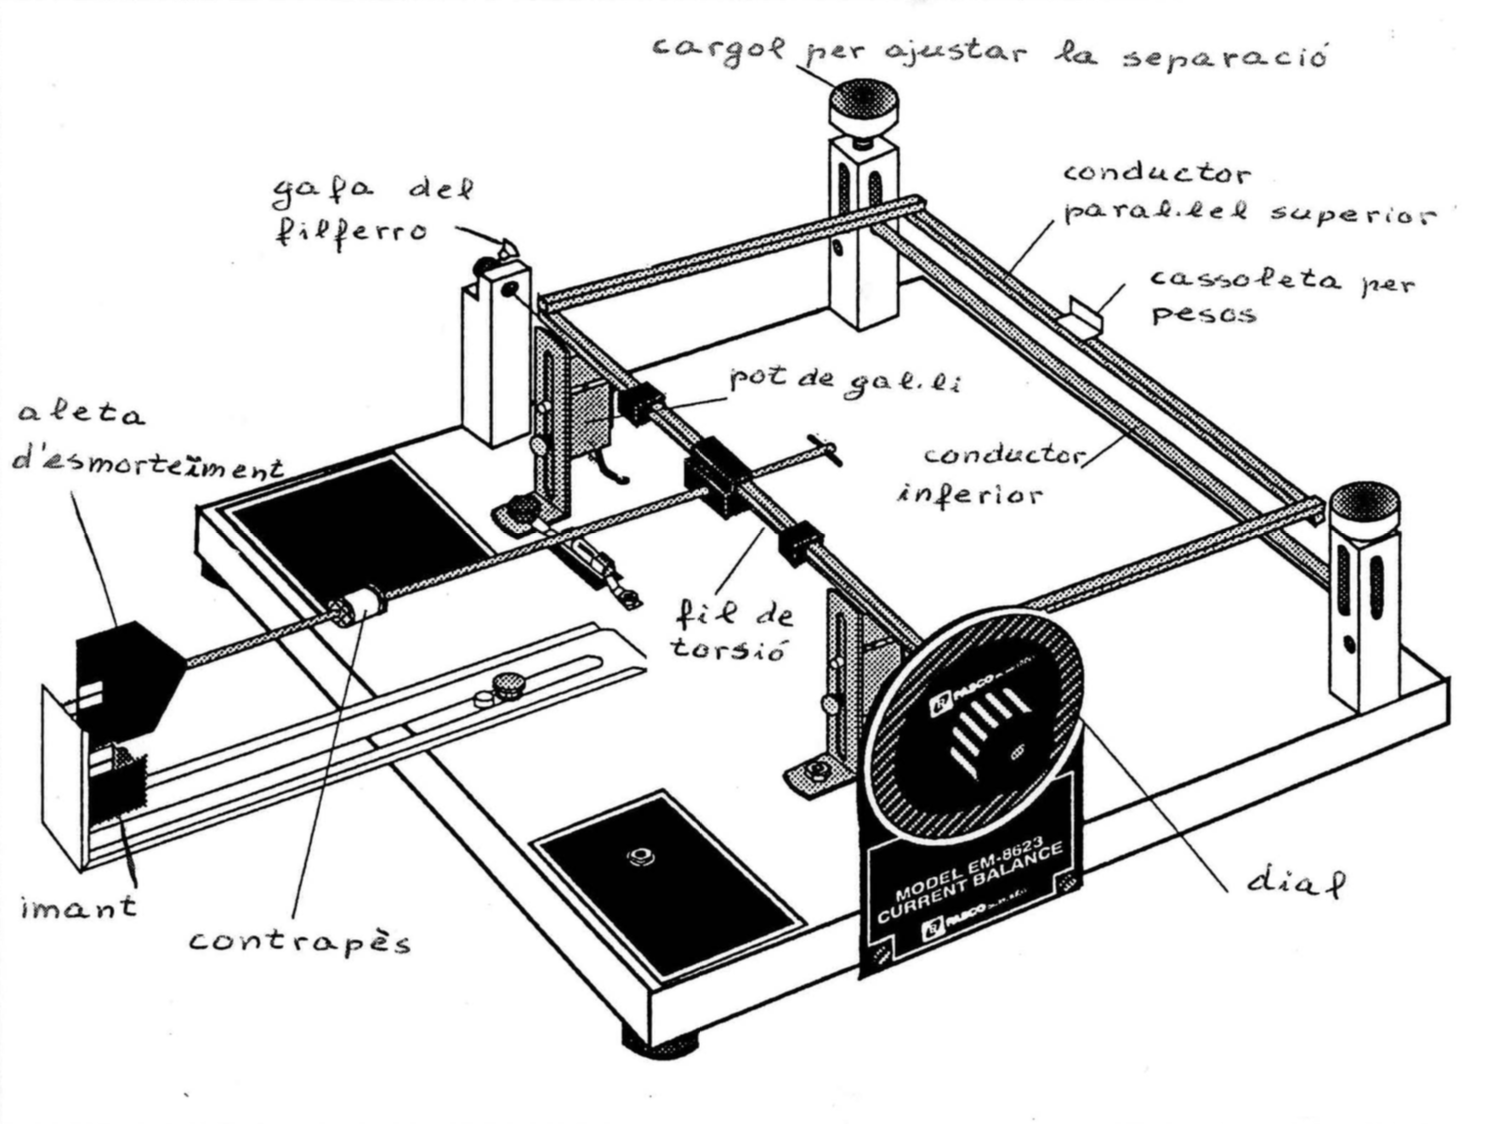
\includegraphics[scale=0.4]{balanca.png}
	\caption{Esquema de la balança de corrents amb els principals elements}
	\label{fig:balanca}
\end{figure}

La balança disposa de dues maneres de determinar la força entre els corrents. Per una banda, disposa d'una cassoleta de pesos on co\l.locar diferents masses. Sabent que, en el moment que la balança es troba equilibrada, la força gravitatòria sobre la massa és igual a la força entre els corrents es pot determinar aquesta última. Per altra banda, la balança també disposa d'un dial i un fil de torsió que poden contrarrestar la força entre els corrents. Sabent que la relació entre els graus que rota el dial i la força que fa és lineal i coneixent la constant de proporcionalitat, es pot determinar també la força entre els corrents.

Cal mencionar que els corrents s'han disposat en direcció nord-sud terrestre per tal que el camp magnètic de la Terra no influís en els resultats.

Cal també comentar que el valor que s'ha pres com a acceleració de la gravetat és \SI{9.80665}{m.s^{-2}} amb incertesa menyspreable en comparació amb la resta d'incerteses que puguin introduir les mesures. S'han pres també sense incertesa els valors de les masses proporcionades al laboratori.

\subsection{Força i intensitat}
Per aquesta part de la pràctica s'ha mesurat la intensitat necessària per compensar la força gravitatòria exercida sobre el cable superior per masses de \SIlist{5; 10; 15; 20; 25}{mg}, un cop havent fixat la distància entre corrents en \SI{8.1}{mm}. Posteriorment s'ha aplicat una regressió lineal entre la força i el quadrat de la intensitat per comprovar la relació predita per l'\cref{eq:forca i corrent}.

\subsection{Força i distància}
En aquesta part, s'ha fixat una intensitat i s'ha anat variant la distància entre els cables. Per cada distància desitjada s'ha determinat la força entre els corrents a partir del mecanisme el fil de torsió. Amb les dades preses s'ha fet una regressió lineal entre la força i l'invers de la distància per verificar la relació predita per l'\cref{eq:forca i corrent} A partir del pendent obtingut en la regressió i l'\cref{eq:forca i corrent} s'ha determinat experimentalment la constant $\mu_0$.

\subsection{Camp magnètic terrestre}
Per aquesta part de l'experiment %Arnau I lof u
s'han orientat els fils en direcció est-oest de manera que fossin perpendiculars al camp magnètic terrestre ---podem, en bona aproximació, suposar que és constant i en la direcció nord-sud---. 

Posteriorment, s'ha fet circular una intensitat fixa només pel fil superior i s'ha determinat la força que patia a través del dial i el fil de torsió. El camp magnètic s'ha determinat a partir de l'\cref{eq:forca magnetica}. 

Com que la força magnètica sobre un fil que porta una intensitat és perpendicular tant al fil com al camp magnètic que la provoca, la disposició de la balança (on els fils es troben sempre horitzontals i només podem mesurar la força veritcal sobre ells) fa impossible la mesura de la component radial del camp magnètic, ja que requeriríem d'un mètode per mesurar la força horitzontal que pateix el fil.

\section{Resultats}
\subsection{Força i intensitat}
La \cref{tab:forca v intensitat} mostra les mitjanes de les intensitats necessàries per contrarrestar la força gravitatòria de les diferents masses usades, essent la distància entre els fils de \SI{8.1}{mm}. La \cref{tab:forca v intensitat (detall)}	de l'annex mostra totes les dades per a cada massa. 

\begin{table}[htb]
	\sffamily \small
	\centering
	\caption{Intensitat mitjana necessària per contrarrestar la força gravitatòria de cada massa.}
	\label{tab:forca v intensitat}
	\begin{tabular}{SS[table-parse-only]}
		\toprule
		{Massa (\si{mg})} & {Intensitat (\si{A})} \\
		\midrule
		5  & 2.62 \pm 0.10 \\
		10 & 3.62 \pm 0.18 \\
		15 & 4.49 \pm 0.15 \\
		20 & 5.19 \pm 0.18 \\
		25 & 5.8 \pm 0.3 \\
		\bottomrule
	\end{tabular}
\end{table}

\begin{figure} [htb]
	\centering \small \sffamily
	% GNUPLOT: LaTeX picture with Postscript
\begingroup
\sffamily \small
  \makeatletter
  \providecommand\color[2][]{%
    \GenericError{(gnuplot) \space\space\space\@spaces}{%
      Package color not loaded in conjunction with
      terminal option `colourtext'%
    }{See the gnuplot documentation for explanation.%
    }{Either use 'blacktext' in gnuplot or load the package
      color.sty in LaTeX.}%
    \renewcommand\color[2][]{}%
  }%
  \providecommand\includegraphics[2][]{%
    \GenericError{(gnuplot) \space\space\space\@spaces}{%
      Package graphicx or graphics not loaded%
    }{See the gnuplot documentation for explanation.%
    }{The gnuplot epslatex terminal needs graphicx.sty or graphics.sty.}%
    \renewcommand\includegraphics[2][]{}%
  }%
  \providecommand\rotatebox[2]{#2}%
  \@ifundefined{ifGPcolor}{%
    \newif\ifGPcolor
    \GPcolortrue
  }{}%
  \@ifundefined{ifGPblacktext}{%
    \newif\ifGPblacktext
    \GPblacktextfalse
  }{}%
  % define a \g@addto@macro without @ in the name:
  \let\gplgaddtomacro\g@addto@macro
  % define empty templates for all commands taking text:
  \gdef\gplbacktext{}%
  \gdef\gplfronttext{}%
  \makeatother
  \ifGPblacktext
    % no textcolor at all
    \def\colorrgb#1{}%
    \def\colorgray#1{}%
  \else
    % gray or color?
    \ifGPcolor
      \def\colorrgb#1{\color[rgb]{#1}}%
      \def\colorgray#1{\color[gray]{#1}}%
      \expandafter\def\csname LTw\endcsname{\color{white}}%
      \expandafter\def\csname LTb\endcsname{\color{black}}%
      \expandafter\def\csname LTa\endcsname{\color{black}}%
      \expandafter\def\csname LT0\endcsname{\color[rgb]{1,0,0}}%
      \expandafter\def\csname LT1\endcsname{\color[rgb]{0,1,0}}%
      \expandafter\def\csname LT2\endcsname{\color[rgb]{0,0,1}}%
      \expandafter\def\csname LT3\endcsname{\color[rgb]{1,0,1}}%
      \expandafter\def\csname LT4\endcsname{\color[rgb]{0,1,1}}%
      \expandafter\def\csname LT5\endcsname{\color[rgb]{1,1,0}}%
      \expandafter\def\csname LT6\endcsname{\color[rgb]{0,0,0}}%
      \expandafter\def\csname LT7\endcsname{\color[rgb]{1,0.3,0}}%
      \expandafter\def\csname LT8\endcsname{\color[rgb]{0.5,0.5,0.5}}%
    \else
      % gray
      \def\colorrgb#1{\color{black}}%
      \def\colorgray#1{\color[gray]{#1}}%
      \expandafter\def\csname LTw\endcsname{\color{white}}%
      \expandafter\def\csname LTb\endcsname{\color{black}}%
      \expandafter\def\csname LTa\endcsname{\color{black}}%
      \expandafter\def\csname LT0\endcsname{\color{black}}%
      \expandafter\def\csname LT1\endcsname{\color{black}}%
      \expandafter\def\csname LT2\endcsname{\color{black}}%
      \expandafter\def\csname LT3\endcsname{\color{black}}%
      \expandafter\def\csname LT4\endcsname{\color{black}}%
      \expandafter\def\csname LT5\endcsname{\color{black}}%
      \expandafter\def\csname LT6\endcsname{\color{black}}%
      \expandafter\def\csname LT7\endcsname{\color{black}}%
      \expandafter\def\csname LT8\endcsname{\color{black}}%
    \fi
  \fi
    \setlength{\unitlength}{0.0500bp}%
    \ifx\gptboxheight\undefined%
      \newlength{\gptboxheight}%
      \newlength{\gptboxwidth}%
      \newsavebox{\gptboxtext}%
    \fi%
    \setlength{\fboxrule}{0.5pt}%
    \setlength{\fboxsep}{1pt}%
\begin{picture}(5668.00,3400.00)%
    \gplgaddtomacro\gplbacktext{%
      \csname LTb\endcsname%%
      \put(1078,704){\makebox(0,0)[r]{\strut{}\num{0}}}%
      \put(1078,1117){\makebox(0,0)[r]{\strut{}\num{0.05}}}%
      \put(1078,1529){\makebox(0,0)[r]{\strut{}\num{0.1}}}%
      \put(1078,1942){\makebox(0,0)[r]{\strut{}\num{0.15}}}%
      \put(1078,2354){\makebox(0,0)[r]{\strut{}\num{0.2}}}%
      \put(1078,2767){\makebox(0,0)[r]{\strut{}\num{0.25}}}%
      \put(1078,3179){\makebox(0,0)[r]{\strut{}\num{0.3}}}%
      \put(1210,484){\makebox(0,0){\strut{}\num{5}}}%
      \put(1790,484){\makebox(0,0){\strut{}\num{10}}}%
      \put(2370,484){\makebox(0,0){\strut{}\num{15}}}%
      \put(2950,484){\makebox(0,0){\strut{}\num{20}}}%
      \put(3531,484){\makebox(0,0){\strut{}\num{25}}}%
      \put(4111,484){\makebox(0,0){\strut{}\num{30}}}%
      \put(4691,484){\makebox(0,0){\strut{}\num{35}}}%
      \put(5271,484){\makebox(0,0){\strut{}\num{40}}}%
      \put(4111,1529){\makebox(0,0){\strut{}$r^2$ = \num{0.999}}}%
    }%
    \gplgaddtomacro\gplfronttext{%
      \csname LTb\endcsname%%
      \put(198,1941){\rotatebox{-270}{\makebox(0,0){\strut{}$\mathsf{F \ (\si{mN})}$}}}%
      \put(3240,154){\makebox(0,0){\strut{}$\mathsf{I^2 \ (\si{A})}$}}%
    }%
    \gplbacktext
    \put(0,0){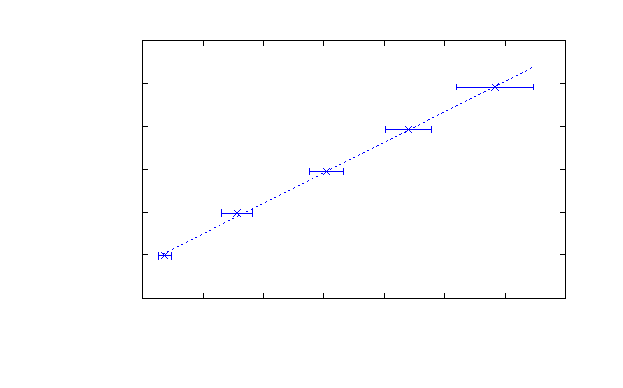
\includegraphics{forca-intensitat}}%
    \gplfronttext
  \end{picture}%
\endgroup

	\caption{Força en funció del quadrat del corrent}
	\label{fig:forca v intensitat}
\end{figure}

Amb els valors presentats a la \cref{tab:forca v intensitat} s'ha fet una regressió lineal entre la força entre corrents i el quadrat de la intensitat, \cref{fig:forca v intensitat}. 

El valor obtingut del pendent de la recta de regressió es de \( \data{7.35}{0.08d-6}{N.A^{-2}} \). A partir d'aquest valor i l'\cref{eq:forca i corrent} s'ha determinat \( \mu_0 = \data{1.25}{0.04d-6}{N.A^{-2}} \) que és compatible amb el valor tabulat, per entrar en el rang d'incerteses i tenir un percentatge d'error petit, del $0.6\%$.

\subsection{Força i distància}
Primerament, a través d'una regressió lineal amb un factor de correlació $r^2=0.985$ s'ha determinat la dependència lineal entre la força exercida pel fil de torsió i la rotació del dial, amb un valor de la constant de proporcionalitat de \( k = \data{3.2}{0.2d-7}{N} \). Les dades de la regressió es poden veure a la \cref{tab:regressio forca-angle} i a la \cref{fig:forca v rotacio}. Així, la força es pot determinar per
\begin{equation} \label{eq:forca i angle}
	F=k\theta
\end{equation}

S'ha fixat una intensitat constant de \( I = \data{5.37}{0.02}{A} \) i s'ha mesurat la rotació necessària del dial per contrarrestrar la força entre corrents. La \cref{tab:forca v desplacament} mostra els resultats. 

\begin{table}[htb]
	\sffamily \small
	\centering
	\caption{Rotació del dial necessària per contrarrestar la força entre corrents a diferents distàncies. La intensitat, fixa, és de \( I = \data{5.37}{0.02}{A} \).}
	\label{tab:forca v desplacament}
	\begin{tabular}{SS}
		\toprule
		{Separació (\data{}{0.001}{m})} &  {Rotació (\data{}{1}{\degree})} \\
		\midrule 
		0.010 & 64 \\ 
		0.009 & 63 \\  
		0.008 & 65 \\  
		0.007 & 87 \\  
		0.006 & 129 \\   
		0.005 & 186 \\   
		\bottomrule
	\end{tabular}
\end{table}

Amb les dades de la \cref{tab:forca v desplacament} s'ha realitzat una regressió lineal entre la força entre corrents, calculada a partir de l'\cref{eq:forca i angle}, i l'invers de la distància, \cref{fig:forca v distancia}.

\begin{figure}[htb]
	\centering
	% GNUPLOT: LaTeX picture with Postscript
\begingroup
\sffamily \small
  \makeatletter
  \providecommand\color[2][]{%
    \GenericError{(gnuplot) \space\space\space\@spaces}{%
      Package color not loaded in conjunction with
      terminal option `colourtext'%
    }{See the gnuplot documentation for explanation.%
    }{Either use 'blacktext' in gnuplot or load the package
      color.sty in LaTeX.}%
    \renewcommand\color[2][]{}%
  }%
  \providecommand\includegraphics[2][]{%
    \GenericError{(gnuplot) \space\space\space\@spaces}{%
      Package graphicx or graphics not loaded%
    }{See the gnuplot documentation for explanation.%
    }{The gnuplot epslatex terminal needs graphicx.sty or graphics.sty.}%
    \renewcommand\includegraphics[2][]{}%
  }%
  \providecommand\rotatebox[2]{#2}%
  \@ifundefined{ifGPcolor}{%
    \newif\ifGPcolor
    \GPcolortrue
  }{}%
  \@ifundefined{ifGPblacktext}{%
    \newif\ifGPblacktext
    \GPblacktextfalse
  }{}%
  % define a \g@addto@macro without @ in the name:
  \let\gplgaddtomacro\g@addto@macro
  % define empty templates for all commands taking text:
  \gdef\gplbacktext{}%
  \gdef\gplfronttext{}%
  \makeatother
  \ifGPblacktext
    % no textcolor at all
    \def\colorrgb#1{}%
    \def\colorgray#1{}%
  \else
    % gray or color?
    \ifGPcolor
      \def\colorrgb#1{\color[rgb]{#1}}%
      \def\colorgray#1{\color[gray]{#1}}%
      \expandafter\def\csname LTw\endcsname{\color{white}}%
      \expandafter\def\csname LTb\endcsname{\color{black}}%
      \expandafter\def\csname LTa\endcsname{\color{black}}%
      \expandafter\def\csname LT0\endcsname{\color[rgb]{1,0,0}}%
      \expandafter\def\csname LT1\endcsname{\color[rgb]{0,1,0}}%
      \expandafter\def\csname LT2\endcsname{\color[rgb]{0,0,1}}%
      \expandafter\def\csname LT3\endcsname{\color[rgb]{1,0,1}}%
      \expandafter\def\csname LT4\endcsname{\color[rgb]{0,1,1}}%
      \expandafter\def\csname LT5\endcsname{\color[rgb]{1,1,0}}%
      \expandafter\def\csname LT6\endcsname{\color[rgb]{0,0,0}}%
      \expandafter\def\csname LT7\endcsname{\color[rgb]{1,0.3,0}}%
      \expandafter\def\csname LT8\endcsname{\color[rgb]{0.5,0.5,0.5}}%
    \else
      % gray
      \def\colorrgb#1{\color{black}}%
      \def\colorgray#1{\color[gray]{#1}}%
      \expandafter\def\csname LTw\endcsname{\color{white}}%
      \expandafter\def\csname LTb\endcsname{\color{black}}%
      \expandafter\def\csname LTa\endcsname{\color{black}}%
      \expandafter\def\csname LT0\endcsname{\color{black}}%
      \expandafter\def\csname LT1\endcsname{\color{black}}%
      \expandafter\def\csname LT2\endcsname{\color{black}}%
      \expandafter\def\csname LT3\endcsname{\color{black}}%
      \expandafter\def\csname LT4\endcsname{\color{black}}%
      \expandafter\def\csname LT5\endcsname{\color{black}}%
      \expandafter\def\csname LT6\endcsname{\color{black}}%
      \expandafter\def\csname LT7\endcsname{\color{black}}%
      \expandafter\def\csname LT8\endcsname{\color{black}}%
    \fi
  \fi
    \setlength{\unitlength}{0.0500bp}%
    \ifx\gptboxheight\undefined%
      \newlength{\gptboxheight}%
      \newlength{\gptboxwidth}%
      \newsavebox{\gptboxtext}%
    \fi%
    \setlength{\fboxrule}{0.5pt}%
    \setlength{\fboxsep}{1pt}%
\begin{picture}(5668.00,3400.00)%
    \gplgaddtomacro\gplbacktext{%
      \csname LTb\endcsname%%
      \put(946,704){\makebox(0,0)[r]{\strut{}\num{0.1}}}%
      \put(946,1117){\makebox(0,0)[r]{\strut{}\num{0.2}}}%
      \put(946,1529){\makebox(0,0)[r]{\strut{}\num{0.3}}}%
      \put(946,1942){\makebox(0,0)[r]{\strut{}\num{0.4}}}%
      \put(946,2354){\makebox(0,0)[r]{\strut{}\num{0.5}}}%
      \put(946,2766){\makebox(0,0)[r]{\strut{}\num{0.6}}}%
      \put(946,3179){\makebox(0,0)[r]{\strut{}\num{0.7}}}%
      \put(1078,484){\makebox(0,0){\strut{}\num{80}}}%
      \put(1677,484){\makebox(0,0){\strut{}\num{100}}}%
      \put(2276,484){\makebox(0,0){\strut{}\num{120}}}%
      \put(2875,484){\makebox(0,0){\strut{}\num{140}}}%
      \put(3474,484){\makebox(0,0){\strut{}\num{160}}}%
      \put(4073,484){\makebox(0,0){\strut{}\num{180}}}%
      \put(4672,484){\makebox(0,0){\strut{}\num{200}}}%
      \put(5271,484){\makebox(0,0){\strut{}\num{220}}}%
    }%
    \gplgaddtomacro\gplfronttext{%
      \csname LTb\endcsname%%
      \put(198,1941){\rotatebox{-270}{\makebox(0,0){\strut{}$\mathsf{F \ (\si{mN})}$}}}%
      \put(3174,154){\makebox(0,0){\strut{}$\mathsf{1/r \ (\si{m^{-1}})}$}}%
    }%
    \gplbacktext
    \put(0,0){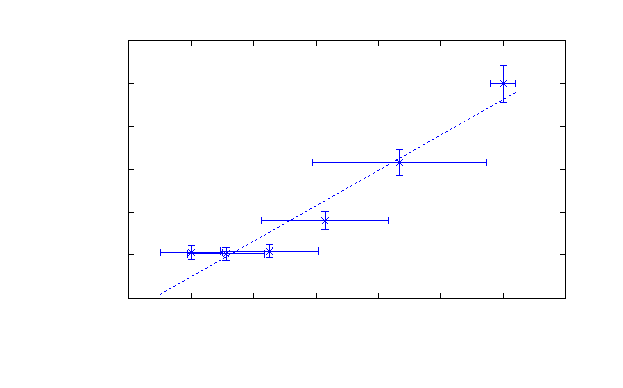
\includegraphics{forca-distancia}}%
    \gplfronttext
  \end{picture}%
\endgroup

	\caption{Força en funció de l'invers de la separació}
	\label{fig:forca v distancia}
\end{figure}

El pendent obtingut a partir de la regressió és \( \data{4.1}{0.6d-6}{N.m} \). A partir d'aquest valor i l'\cref{eq:forca magnetica} s'ha determinat experimentalment el valor de la constant \( \mu_0 = \data{3.0}{0.4d-6}{N.A^{-2}} \). Tenint en compte que el valor teòric de $\mu_0= \SI{1.257e-6}{N.m}$, llavors la mesura té un percentatge d'error del $58\%$. Per tant el resultat no és consistent amb el valor tabulat, possiblement per interferències amb altres elements, però sí de l'orde del valor acceptat.

\subsection{Camp Magnètic Terrestre}
La \cref{tab:camp terrestre} mostra tres mesures d'intensitat i les respectives rotacions del dial per tal de compensar la força que el cable pateix degut a la component radial del camp magnètic terrestre. La força s'obté a partir de l'\cref{eq:forca i angle}, i el camp a partir de l'\cref{eq:forca i corrent}.

\begin{table}[htb]
	\sffamily \small
	\centering
	\caption{Mesures de la component radial del camp magnètic terrestre}
	\label{tab:camp terrestre}
	\begin{tabular}{SSS[table-parse-only]}
		\toprule
		{Intensitat (\data{}{0.01}{A}) } & {Rotació (\data{}{0.01}{\degree}) } & {Camp magnètic (\SI{e-5}{T})} \\
		\midrule
		6.06 & 8& 1.4 \pm 0.3 \\
		6.13 & 8  & 1.4 \pm 0.3 \\
		6.57 & 12 & 2.0 \pm 0.4 \\ 
		\bottomrule
	\end{tabular}
\end{table}

D'aquesta manera, obtenim, a partir de la mitjana aritmètica dels valors de la \cref{tab:camp terrestre}, un valor de la component radial del camp magnètic terrestre de \( B = \data{1.59}{0.18d-5}{T}  \). El resultat no és consistent amb el valor tabulat del camp magnètic a Madrid l'any 1975, possiblement per interferències amb altres elements, però sí que n'és de l'ordre.

\section{Conclusions}
Aquesta experiència s'ha realitzat prenent mesures en una balança de corrents, que permet obtenir la força magnètica que s'exerceixen dos fils para\l.lels suportant intensitats iguals a partir del pes de certes masses o de la rotació d'un dial connectat a un fil de torsió.

Els resultats obtinguts demostren experimentalment la relació lineal entre la força magnètica que s'exerceixen dos fils para\l.lels pels quals hi circula la matreixa intensitat i el quadrat d'aquesta intensitat, així com entre la força i l'invers de la distància entre els fils.

Els experiments també han permès determinar experimentalment la constant $\mu_0$, obtenint valors de \( \mu_0 = \data{1.25}{0.04e-6}{N.A^{-2}} \) i \( \mu_0 = \data{3.0}{0.4d-6}{N.A^{-2}} \). Mentre que el primer és consistent amb el valor tabulat, el segon només n'és de l'ordre. Cal mencionar que la qualitat de la regressió de la \cref{fig:forca v intensitat} és molt millor que la de la \cref{fig:forca v distancia}, i això es veu reflectit en el valor de \( \mu_0 \) obtingut a partir de cada una. 

Finalment, s'ha pogut mesurar la component horitzontal del camp magnètic terrestre, també amb l'ajuda de la balança de corrents, obtenint \( B = \data{1.59}{0.18d-5}{T} \). Aquesta mesura, tot i estar molt possiblement contaminada per soroll i altres efectes del laboratori, és consistent amb l'ordre de magnitud que descriuen altres articles. 
